\documentclass[letterpaper,draft]{memoir}
\usepackage[final]{microtype}
% Use [final] to include the graphics despite [draft] above.
\usepackage[final]{graphicx}
\usepackage{gradientframe}
%\usepackage{xcolor}
%\usepackage{pstricks,pst-grad,pst-slpe}
\usepackage[latin,german,greek,english]{babel}
\usepackage[small]{caption}
\usepackage{framed}
\usepackage{makeidx}
\usepackage[english]{isodate}
\usepackage{fullpage}
\usepackage[explicit]{titlesec}
\usepackage[utf8x]{inputenc}
\usepackage{eso-pic}
\usepackage{textcomp}

\makeindex

\makeatletter
\renewcommand{\@pnumwidth}{1.75em}
\renewcommand{\@tocrmarg}{2.75em}
\makeatother

\ifdraftdoc
\makeoddfoot{plain}{\textbf{\tiny\LaTeX\ draft: \today}}{\normalsize \textcircled{\scriptsize \thepage}}{\tiny Copyright \copyright\ 2012 Nick Black}
\makeevenfoot{plain}{\tiny Copyright \copyright\ 2012 Nick Black}{\normalsize \textcircled{\scriptsize \thepage}}{\textbf{\tiny \LaTeX\ draft: \today}}
\fi

\captionsetup{font=scriptsize,labelfont=scriptsize}

\makeatletter
\def\maketitle{%
  \null
  \thispagestyle{empty}
\begin{leftbar}
  \begin{center}
    \normalfont
    {\huge\raggedleft\@title\par}%
    \hrulefill\par
    {\LARGE\raggedleft\@author\par}%
    \begin{center}
	    \gradientframe{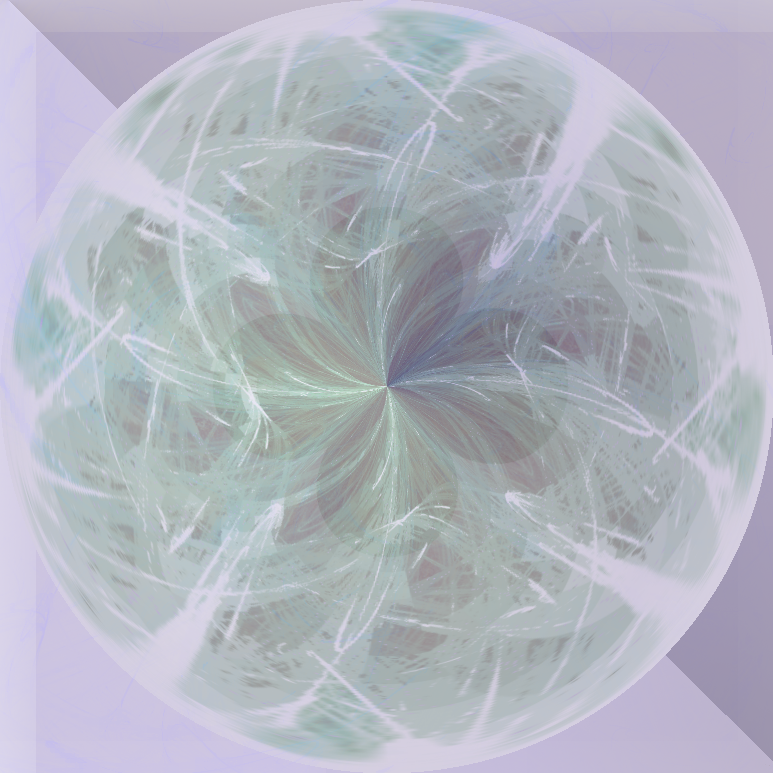
\includegraphics[width=6in]{background.png}}
    \end{center}
  \end{center}%
\end{leftbar}
  \vfill
  \null
  \clearpage
}
\makeatother
\author{nick black}
\title{\emph{\textbf{the finest machine}}\\
\normalsize the science and the joy of computing}
\date{2012}

\newcommand*\Hide{%
\titleformat{\section}
  {}{}{0pt}{}
\titleformat{\chapter}
  {}{}{0pt}{}
\titleformat{\part}
  {}{}{0pt}{}
}

\isodate

\begin{document}
\frenchspacing
\maketitle

\pagecolor{white}


%\thispagestyle{empty}
{
\Hide
\section{DEDICATION}
}
\noindent DEDICATED to my professors, my students, and my friends at the Georgia Institute of Technology, who give rise
to that spirit living \textit{in his machinis ex deis}. Hack on, lads, hack on!\\

\noindent TO ALL THOSE who took a wary chance on a risky bet, especially Coach Jeanette
Martin: thanks for everything. You made possible this work of tightly-controlled
audacity. \textit{Per ardua ad astra}.\\

\raggedleft\footnotesize{---Atlanta, 2012}

\vspace{6in}

\center\scriptsize{\textbf{This document was prepared on Debian Linux using \LaTeX, the GIMP, ImageMagick, GNU Make, and Vim.}}
\center\tiny{Debian is a registered trademark of Software in the Public Interest, Inc.\\ImageMagick is a registered trademark of ImageMagick Studio LLC.}
\clearpage

\raggedleft\footnotesize

%\thispagestyle{empty}
\begin{quote}I made a discovery today. I found a computer\ldots And then it happened\ldots a door
opened to a world\ldots rushing through the phone line like heroin through an
addict's veins, an electronic pulse is sent out, a refuge from the
day-to-day\ldots This is it, this is where I belong.\\
\raggedleft{\tiny---The Mentor, ``The Hacker Manifesto''\\
\emph{Phrack} Vol.\ One, Issue Seven, Phile 3 (\printdate{25.09.1986})}
\end{quote}

\vspace{.2in}

\begin{quote}Something else gets under your skin, keeps you working days and nights at the
sacrifice of your sleeping and eating and attention to your family and friends,
something beyond the love of puzzle solving. And that other force is the
anticipation of understanding something about the world that no one has ever
understood before you\ldots I have experienced that pleasure of discovering
something new. It is an exquisite sensation, a feeling of power, a rush of the
blood, a sense of living forever. To be the first vessel to hold this new
thing.

\noindent All of the scientists I've known have at least one more quality in common:
they do what they do because they love it, and because they cannot imagine
doing anything else. In a sense, this is the real reason a scientist does
science. Because the scientist must. Such a compulsion is both blessing and
burden. A blessing because the creative life, in any endeavor, is a gift
filled with beauty and not given to everyone, a burden because the call is
unrelenting and can drown out the rest of life.

\noindent This mixed blessing and burden must be why the astrophysicist Chandrasekhar
continued working until his mid-80's, why a visitor to Einstein's apartment in
Bern found the young physicist rocking his infant with one hand while doing
mathematical calculations with the other. This mixed blessing and burden must
have been the ``sweet hell'' that Walt Whitman referred to when he realized at a
young age that he was destined to be a poet. ``Never more,'' he wrote, ``shall I
escape.''\\
\raggedleft{\tiny---Alan Lightman, ``Spellbound by the Eternal Riddle, Scientists Revel in Their Captivity'',\\
New York Times (\printdate{11.11.2003})}\\
\end{quote}
\vspace{.2in}
\begin{quote}Part of the inhumanity of the computer is that, once it is competently
 programmed and working smoothly, it is completely honest. I do not fear
 computers. I fear the lack of them.\\
\raggedleft{\tiny---Isaac Asimov, source unknown}
\end{quote}
\vspace{.2in}
\begin{quote}Nature does not know extinction; all it knows is transformation. Everything
 science has taught me, and continues to teach me, strengthens my belief in the
 continuity of our spiritual existence.\\
\vspace{2mm}
\raggedleft{\tiny---Wernher Von Braun, ``Why I Believe in Immortality'',\\
from \emph{The Third Book of Words to Live By}, W. Nichols (ed.) (1962)}
\end{quote}
\vspace{.2in}
\begin{quote}In the particular is contained the universal.\\
\raggedleft{\tiny---Anton Chekhov, as quoted by James Joyce in\\
Arthur Power's \emph{From the Old Waterford House} (1949)}
\end{quote}
\vspace{.2in}
\begin{quote}There may indeed be other applications of the system than its use as a logic.\\
\raggedleft{\tiny---Alonzo Church,\\
\emph{The Calculi of Lambda-Conversion} (1932)}
\end{quote}
\clearpage

{
\Hide
\section{PREFACE}
\section{INTRODUCTION\@: For madmen only. Price of admission: your mind.}
}
\addtocontents{toc}{\vspace{.25in}}
\tableofcontents
\clearpage

\part{BEYOND THE ZERO\@.}

\addtocontents{toc}{
\bigskip
\protect\begin{quote}
``\emph{Die ganze Zahl schuf der liebe Gott, alles Ubrige ist Menschenwerk.}'' \protect\\
 (``God made the integers; the rest is the work of man.'')\protect\\
\protect\raggedleft{\footnotesize---Leopold Kronecker, as quoted in H. Weber's\protect\\
``Leopold Kronecker'', \emph{Mathematische Annalen} Vol.\ 43, No.\ 1 (1892)}
\protect\end{quote}
}

\chapter{Countable and uncountable numbers. Diagonalization. Gödel numbering and
semiotics. Formally undecidable propositions and Gödel's Theorem.}

\chapter{Wittgenstein and correspondence theories of truth. Stochastic processes.
Richard's Paradox and the Paradox of Rosser and Kleene.}

\chapter{Digital representation of seemingly analog existence. Advantages of digital
systems. Digital life.}

\chapter{Computable recursive functions. Von Neumann and Harvard architectures.
Circuit complexity. Instruction set architecture. Processor frontends. Real computation.}

\part{THE PHYSICS OF INFORMATION\@.}

\addtocontents{toc}{
\bigskip
\protect\begin{quote}
``All things physical are information-theoretic in origin, and this is a
participatory universe. Observer participancy gives rise to information; and
information gives rise to physics.''\protect\\
\protect\raggedleft{\footnotesize---John Archibald Wheeler, \emph{It from Bit} (1989)}
\protect\end{quote}
}

\chapter{Information theory of Szilard and Shannon. Entropy and negentropy. Periodic
and aperiodic crystals. Digital physics.}

\chapter{Signals. Sampling theory of Nyquist. The Fourier transform.}

\chapter{Time's Arrow and the Second Law of Thermodynamics. Heisenberg's uncertainty
principle. Landauer's principle. The wrath of Maxwell's Demon.}

\chapter{The employ of direct currents. Voltage, frequency, resistance, and capacitance. Semiconductors.}

\chapter{Quantum and optical noise. Leakage and the smallest transistor. Principles
of VLSI\@. Memristors.}

\addtocontents{toc}{\protect\clearpage}

\part{THE ESSENCE AND LIMITS OF COMPUTATION\@.}

\addtocontents{toc}{
\bigskip
\protect\begin{quote}
``All physical systems can be thought of as registering and processing
 information, and how one wishes to define computation will determine your view
 of what computation consists of.''\protect\\
\protect\raggedleft{\footnotesize---Seth Lloyd,\protect\\
``Ultimate Physical Limits to Computation'', \emph{Nature} 406 (\printdate{31.08.2000})}
\protect\end{quote}
}

\chapter{Hierarchy theory of Chomsky. Deterministic and nondeterministic machines.
Turing's Machine, Curry's combinatory logic, and Church's \greektextλ\latintext-calculus. The
Church-Turing Thesis. Information-theoretic limitations of formal systems.}

\chapter{Uncomputable functions. Polynomial and Exponential hierarchies. Reductions
of Karp and Levin. NP-completeness. Machine-oblivious analysis of algorithms.}

\chapter{Fixed and floating point. Counting quickly. Numerical approximations and
stabilities. Well-conditioned algorithms. The bounding, detection, and
correction of errors.}

\chapter{Computation elements. Real algorithm analysis. Brent's Theorem and
Gustafson's Law.}

\chapter{Lloyd's limit. Kolmolgorov complexity, algorithmic information theory and
Chaitin's Constant. Schmidhuber's Super-\greektextΩ \latintext{and Speed Prior.}}

\chapter{Queueing theory of Kleinrock. Baran and distributed communication. Quantum
computing, BQP, and spaces of infinitely many dimensions.}

\chapter{Pseudorandom numbers and pseudorandomized algorithms. The possibility of
reversible computation.}

\chapter{Programming language theory. Compilation. Security and the undecidability of
static analysis.}

\chapter{Code as data. Von Neumann's revenge. Self-modifying code and genetics.
Binding and reduction. The joy of LISP\@. Dijkstra's revenge.}

\part{THE INELUCTABLE MODALITY OF STATE\@.}

\addtocontents{toc}{
\bigskip
\protect\begin{quote} ``\emph{\greektextμεταβάλλον αναπαύεται\latintext.}''\protect\\
 (``Even while it changes, it stands still.'')\protect\\
\protect\raggedleft{\footnotesize---\greektextΉράκλειτος\latintext\ (Heraclitus the Ephesian),
as quoted in Abelson and Sussman's\protect\\
\emph{The Structure and Interpretation of Computer Programs} (Second Edition, 1996)}
\protect\end{quote}
}

\chapter{The persistence of information and remembrance of things past. Search. Data structures.}

\chapter{Communication networks. Hypercubes, butterflies and banyans.}

\chapter{Indexing. Fractal structure and Hausdorff dimension of data. Compression.
Address spaces and content-addressed memories.}

\chapter{Memory architecture. Remembering quickly. Offline and online algorithms.
Infinite representations.}

\chapter{The complexity of state and the nature of time. Spacetime and statetime:
transformations among space, state and time. Is computation energy?}

\chapter{Parallelism among bits, registers, instructions, memories, and threads. The
Taxonomy of Flynn.}

\chapter{Dataflow and transport-triggered architectures. Out-of-order processors.
Coherent and incoherent memories. SMP and NUMA\@.}

\chapter{ACID and relational databases. Transactional memory. Ferromagnetic and
plastico-optical storage. The rotting of bits.}

\addtocontents{toc}{\protect\clearpage}

\part{CONSILIENCE\@.}

\addtocontents{toc}{
\bigskip
\protect\begin{quote}``\emph{Die Welt ist alles, was der Fall ist\ldots Wovon man nicht sprechen kann, darüber muß man schweigen.}''\protect\\
 (``The world is all that is the case. Whereof one cannot speak, one must remain silent.'')\protect\\
\protect\raggedleft{\footnotesize---Ludwig Wittgenstein, \emph{Tractatus Logico-Philosophicus} (1918)}
\protect\end{quote}
}

\chapter{Turing dreams he is a machine.}
\chapter{A machine dreams it is Turing.}
\chapter{Consilience.}

\addtocounter{part}{1}
\addtocounter{chapter}{1}

\addtocontents{toc}{\vspace{.3in}}
\section{AFTERWARD\@: The Finest Machine.}
\cite{Witt18}
\addtocontents{toc}{\vspace{.15in}}

\bibliographystyle{plain}
\bibliography{machines}

%%\clearpage
\addcontentsline{toc}{chapter}{Index}
\chapter*{Index}
\printindex

\addtocontents{toc}{\vspace{1in}
\protect\begin{figure}[htb]
\protect\centering
\protect\gradientframe{\protect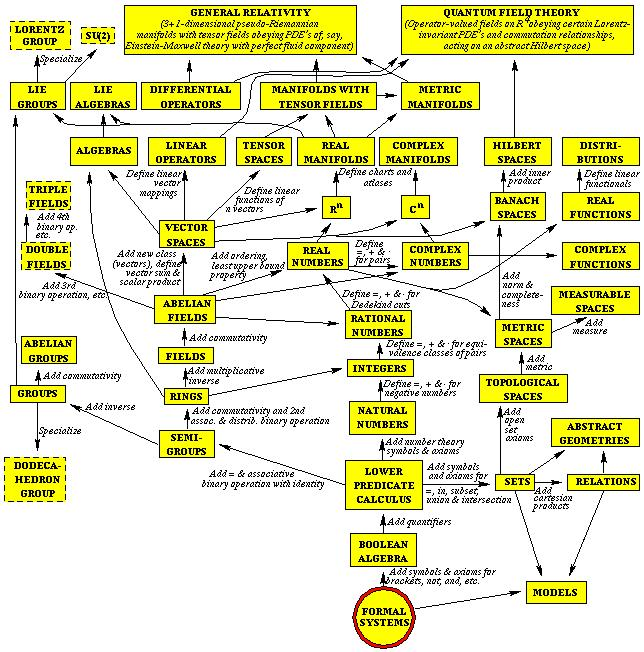
\includegraphics[width=4in,keepaspectratio]{theoryofeverything.jpg}}
\protect\caption{\emph{``What Goes on at the Top?''} Max Tegmark, 2001. Used with permission.}
\protect\end{figure}
}

\end{document}
